\documentclass[letterpaper,12pt,]{article}

\usepackage[%
    left=1in,%
    right=1in,%
    top=1in,%
    bottom=1.0in,%
    paperheight=11in,%
    paperwidth=8.5in%
]{geometry}%

\usepackage{listings}
\usepackage{graphicx}
\usepackage{amsmath}
\usepackage[font=small,skip=-2pt]{caption}
\usepackage{subcaption}
\usepackage{hyperref}
\usepackage{booktabs}
\usepackage{pdfpages}
\usepackage{pgffor}
\usepackage[section]{placeins}


\lstdefinestyle{mystyle}{
    %backgroundcolor=\color{backcolour},
    %commentstyle=\color{codegreen},
    %keywordstyle=\color{magenta},
    %numberstyle=\tiny\color{codegray},
    %stringstyle=\color{codepurple},
    basicstyle=\footnotesize,
    breakatwhitespace=false,
    breaklines=true,
    captionpos=b,
    keepspaces=true,
    numbers=left,
    numberstyle=\footnotesize,
    stepnumber=1,
    numbersep=5pt,
    showspaces=false,
    showstringspaces=false,
    showtabs=false,
    tabsize=2,
    frame=single
}
\lstset{frame=single}

\pagestyle{empty} % Remove page numbering
\linespread{1.5} % Line Spacing

\begin{document}

\begin{titlepage}

\newcommand{\HRule}{\rule{\linewidth}{0.5mm}} % Defines a new command for the horizontal lines, change thickness here

\center % Center everything on the page
 
%----------------------------------------------------------------------------------------
%	HEADING SECTIONS
%----------------------------------------------------------------------------------------


\textsc{\LARGE McGill University}\\[3.5cm]
\textsc{\Large Computational Aerodynamics}\\[0.5cm] 
\textsc{\large MECH 539}\\[2.5cm]

%----------------------------------------------------------------------------------------
%	TITLE SECTION
%----------------------------------------------------------------------------------------

{ \huge \bfseries Final Project}\\[1.5cm] % Title of your document

\HRule \\[0.4cm]
%----------------------------------------------------------------------------------------
%	AUTHOR SECTION
%----------------------------------------------------------------------------------------

\begin{minipage}{0.4\textwidth}
\begin{flushleft} \large
\emph{Name:}\\
Doug \textsc{Shi-Dong} % Your name
\end{flushleft}
\end{minipage}
~
\begin{minipage}{0.4\textwidth}
\begin{flushright} \large
\emph{Student ID:} \\
260466662\\
\end{flushright}
\end{minipage}\\[4cm]

\vfill{}
{\large April 29, 2016}\\[2cm]

\end{titlepage}


\section{Scalar Dissipation - Euler Explicit}

Euler Explicit, Scalar Dissipation of 0.06 and CFL of 0.1 has been used.

\begin{figure}[!ht]
    \centering
    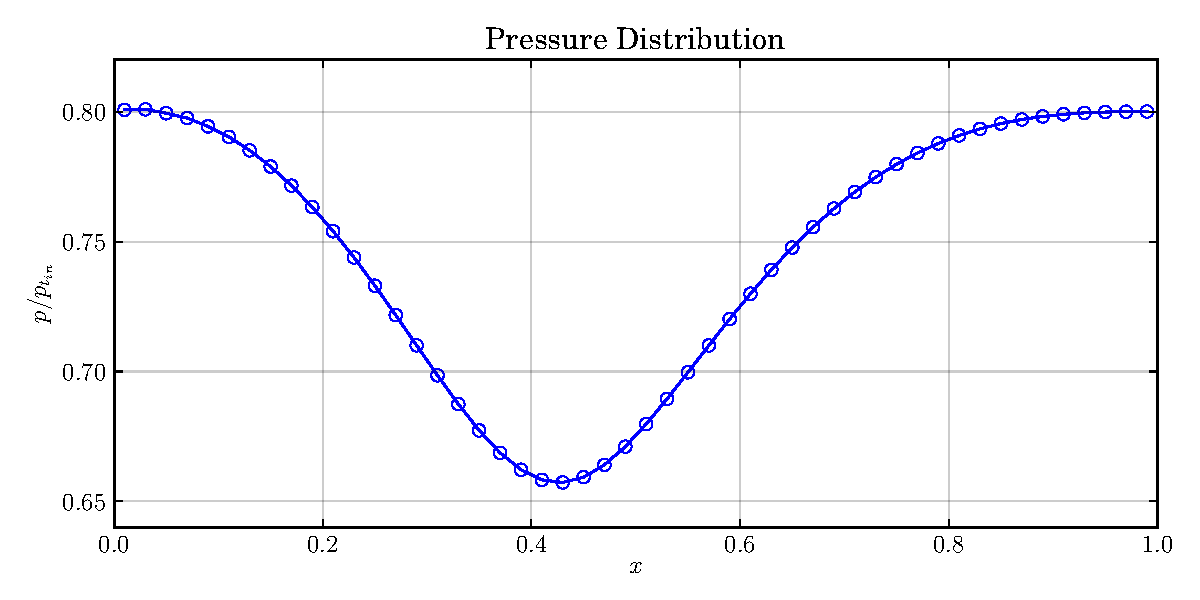
\includegraphics[width = 0.9\textwidth]{./figures/q1p.pdf}
    \caption {Pressure Distribution}
    \label{fig:q1p}
\end{figure}

\begin{figure}[!ht]
    \centering
    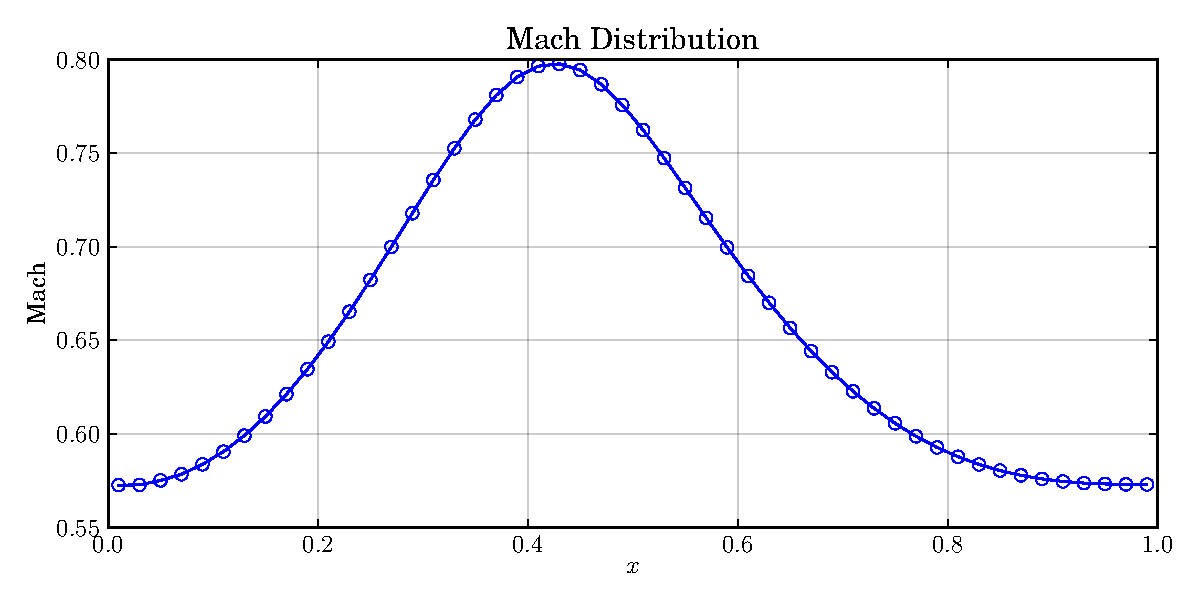
\includegraphics[width = 0.9\textwidth]{./figures/q1m.pdf}
    \caption {Mach Distribution}
    \label{fig:q1m}
\end{figure}

\begin{figure}[!ht]
    \centering
    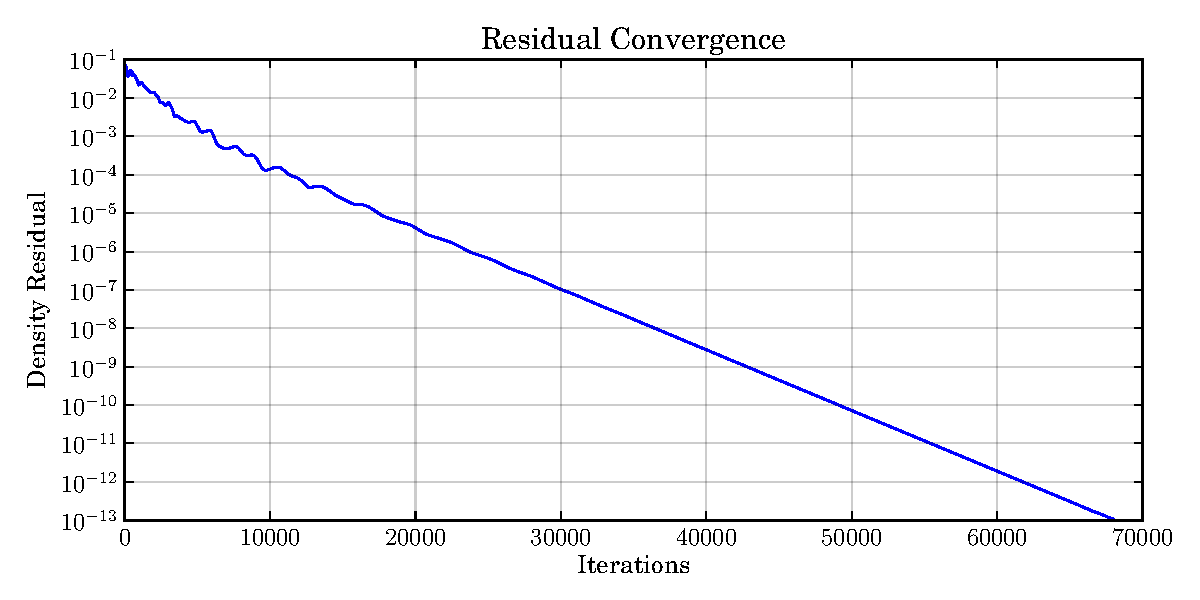
\includegraphics[width = 0.9\textwidth]{./figures/q1c.pdf}
    \caption {Density Residual Convergence}
    \label{fig:q1p}
\end{figure}

\section{Exit Pressure Study}

\begin{figure}[!ht]
    \centering
    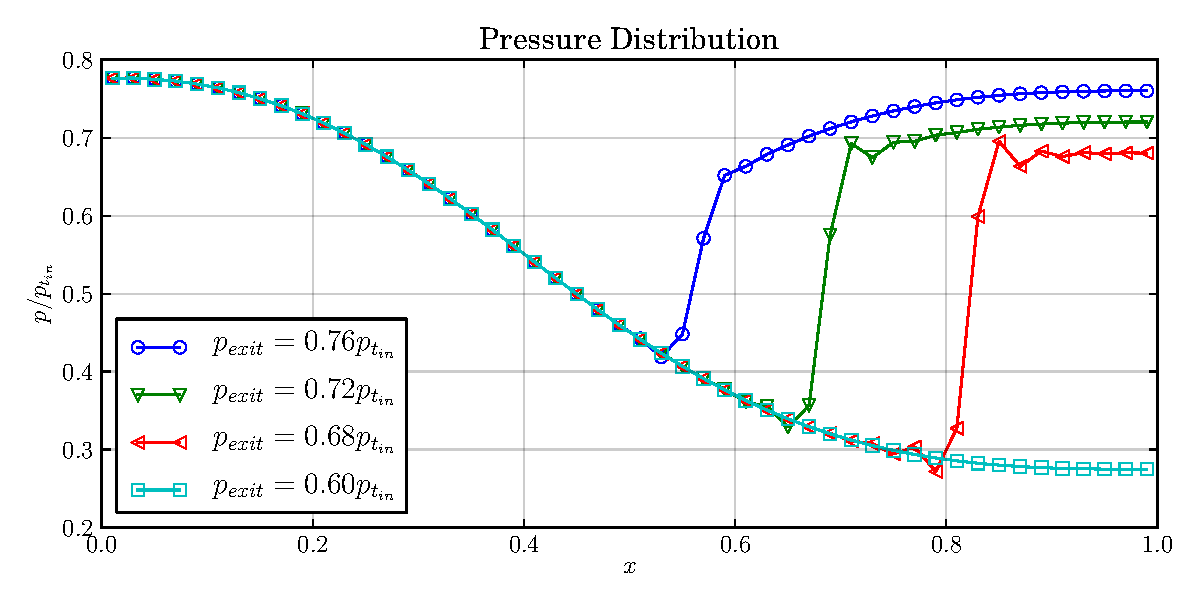
\includegraphics[width = 0.9\textwidth]{./figures/q2p.pdf}
    \caption {Pressure Distribution for Various Exit Pressures}
    \label{fig:q2p}
\end{figure}

\begin{figure}[!ht]
    \centering
    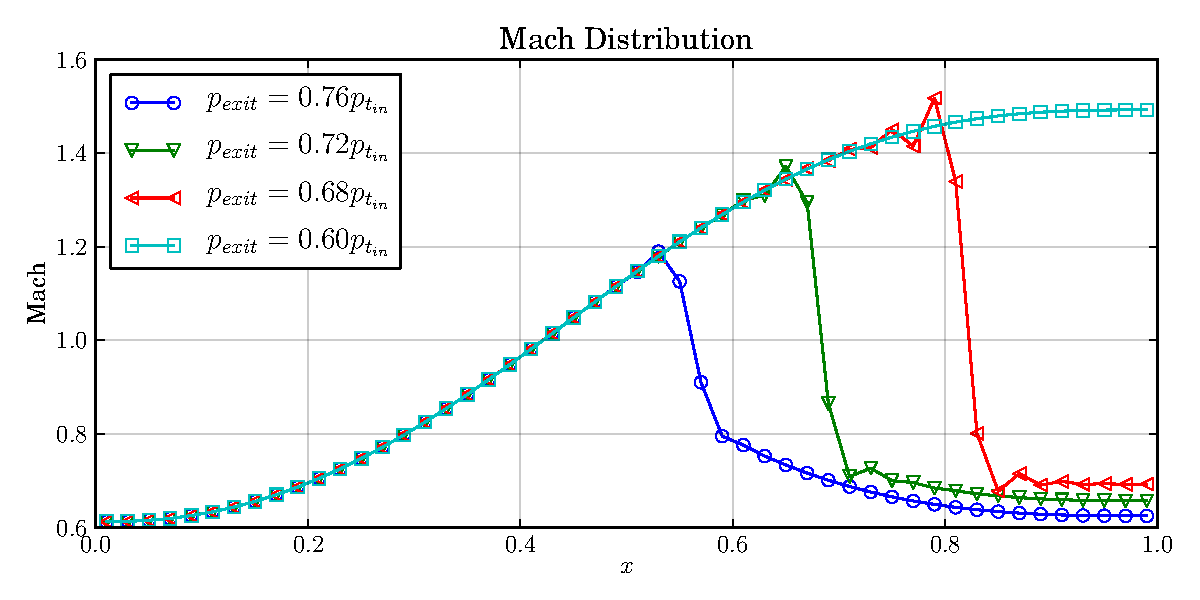
\includegraphics[width = 0.9\textwidth]{./figures/q2m.pdf}
    \caption {Mach Distribution for Various Exit Pressures}
    \label{fig:q2m}
\end{figure}

\begin{figure}[!ht]
    \centering
    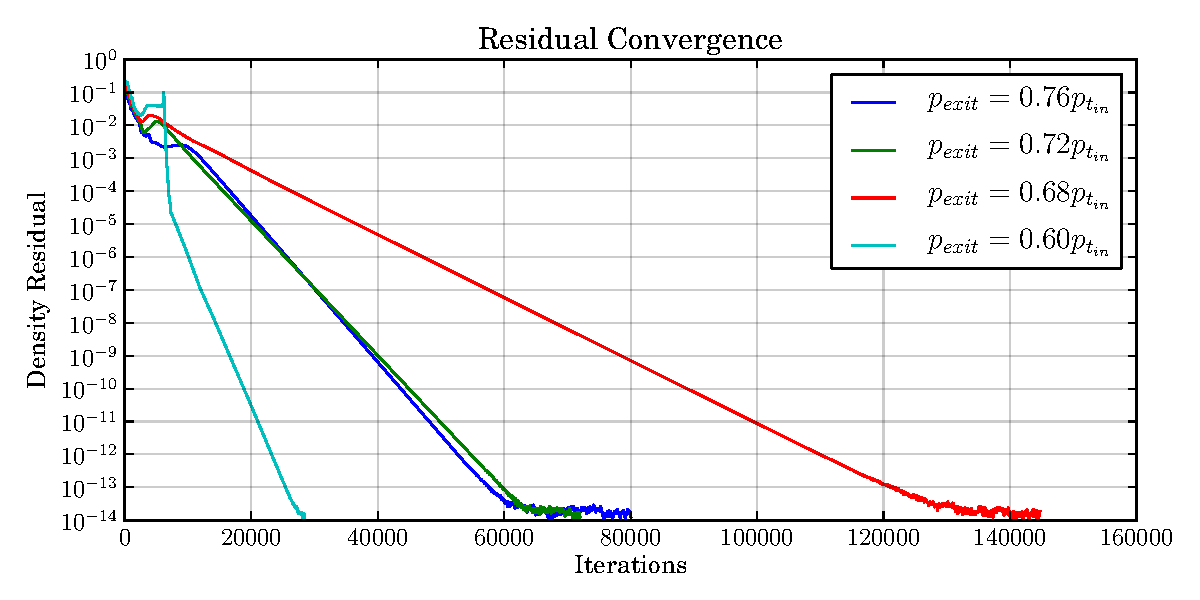
\includegraphics[width = 0.9\textwidth]{./figures/q2c.pdf}
    \caption {Density Residual Convergence for Various Exit Pressures}
    \label{fig:q2p}
\end{figure}

\section{Grid Study}

Euler Explicit, Scalar Dissipation of 0.06 and CFL of 0.1 has been used.

\begin{figure}[!ht]
    \centering
    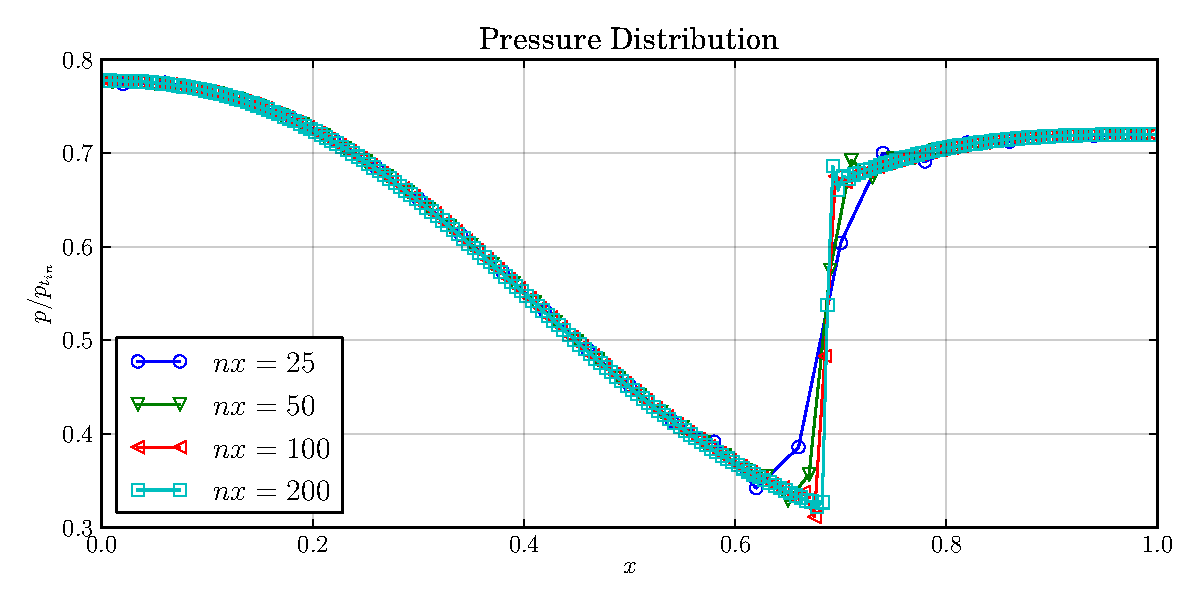
\includegraphics[width = 0.9\textwidth]{./figures/q3p.pdf}
    \caption {Pressure Distribution for Various Grid Sizes}
    \label{fig:q3p}
\end{figure}

\begin{figure}[!ht]
    \centering
    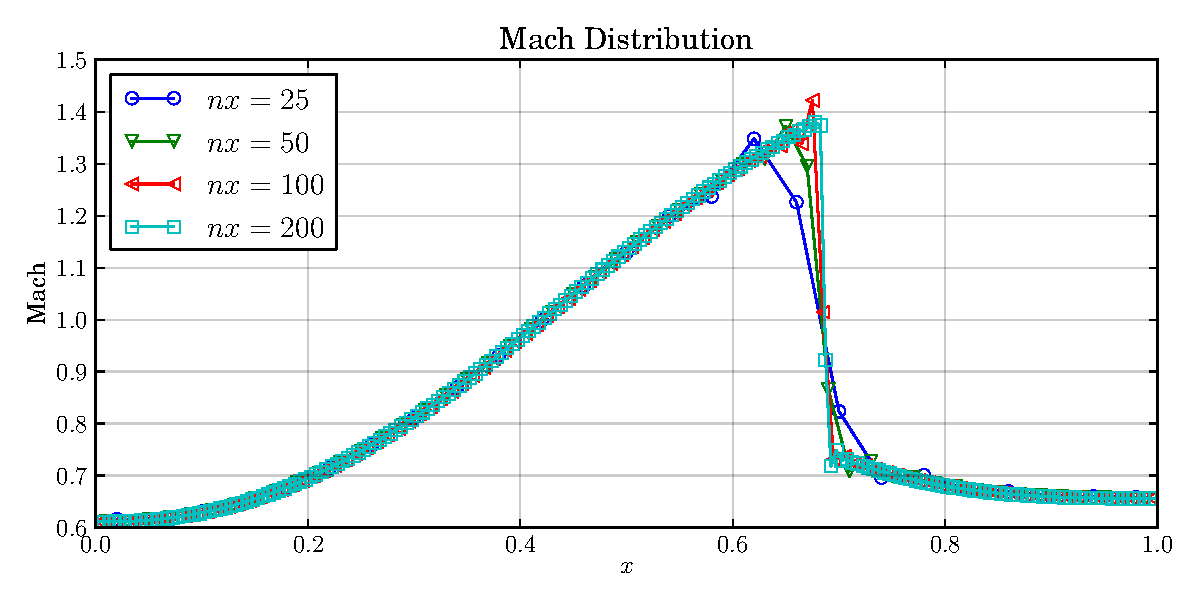
\includegraphics[width = 0.9\textwidth]{./figures/q3m.pdf}
    \caption {Mach Distribution for Various Grid Sizes}
    \label{fig:q3m}
\end{figure}

\begin{figure}[!ht]
    \centering
    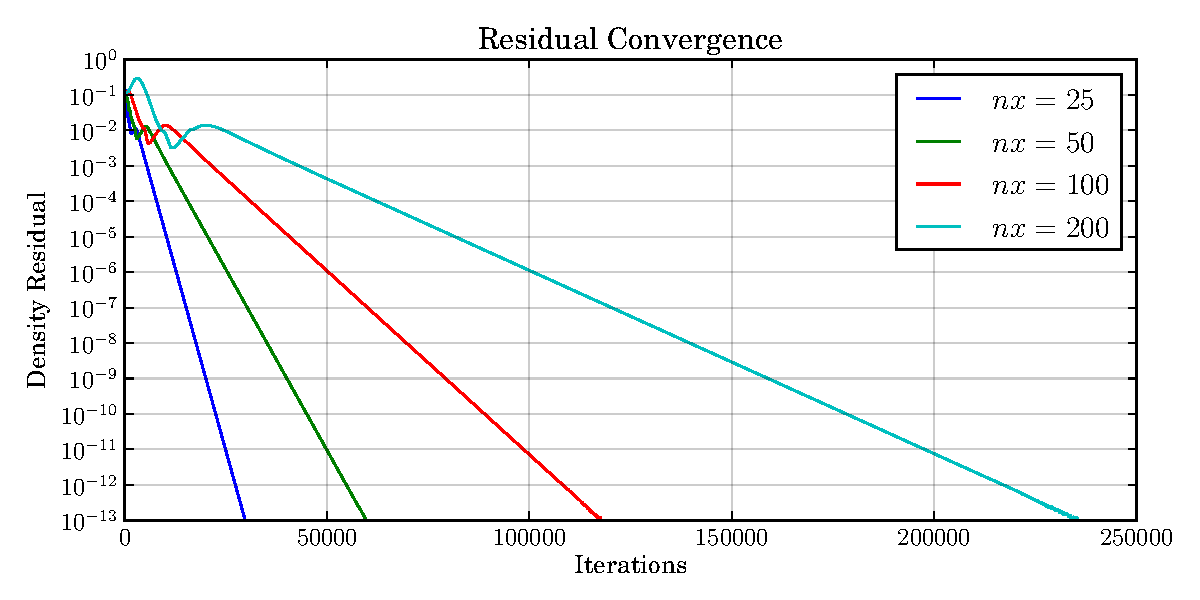
\includegraphics[width = 0.9\textwidth]{./figures/q3c.pdf}
    \caption {Density Residual Convergence for Various Grid Sizes}
    \label{fig:q3p}
\end{figure}

\begin{figure}[!ht]
    \centering
    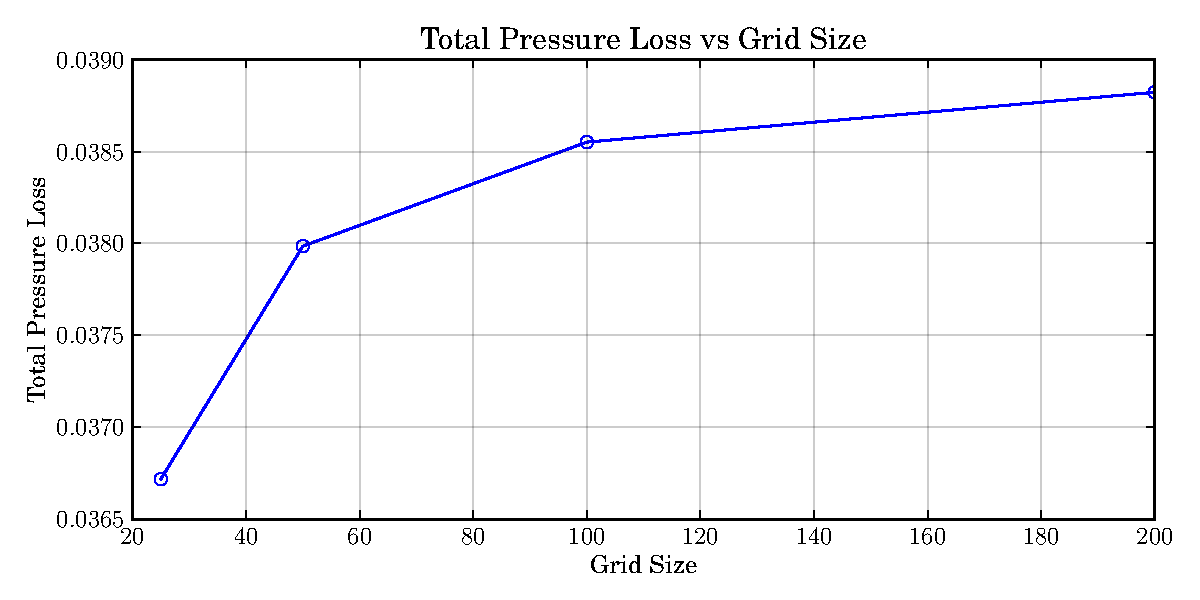
\includegraphics[width = 0.9\textwidth]{./figures/q3loss.pdf}
    \caption {Total Pressure Loss Grid Study}
    \label{fig:q3loss}
\end{figure}

\begin{table}[!h]
\centering
\begin{tabular}{cc} \toprule
    {Number of Grid Points} & {Total Pressure Loss} \\
    \midrule
    {25}  & 0.0367182\\
    {50}  & 0.0379852\\
    {100} & 0.0385511\\
    {200} & 0.0388222\\
\bottomrule
\end{tabular}
\caption{Total Pressure Loss for Various Grid Sizes}
\label{tab1}
\end{table}

\section{Flux Discretization Study}

Euler Explicit and CFL of 0.1 has been used.

\begin{figure}[!ht]
    \centering
    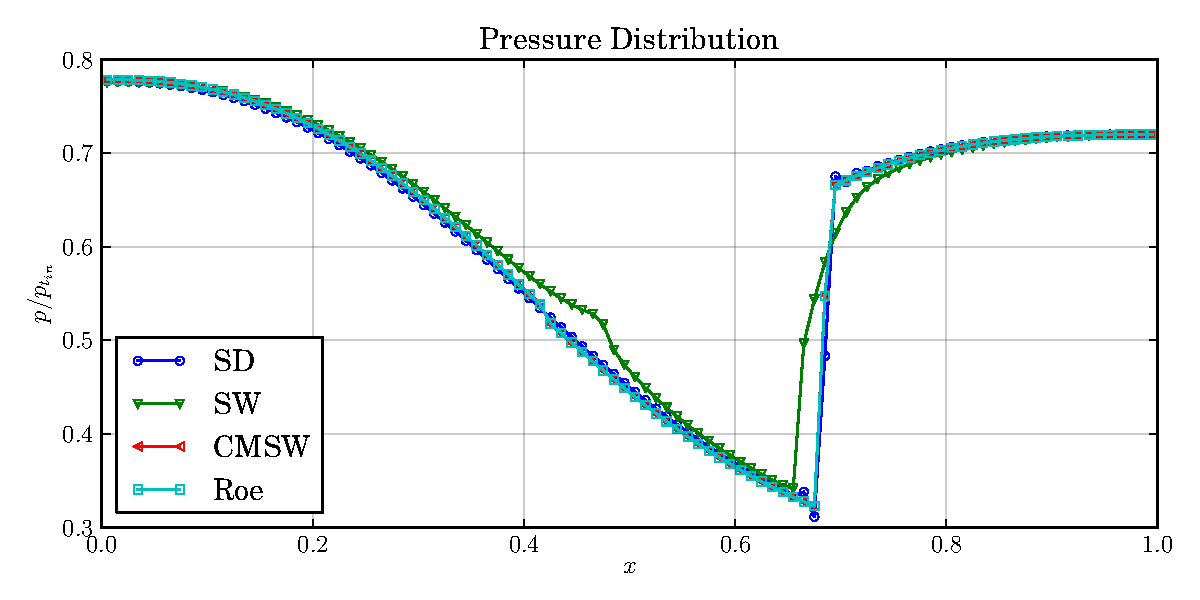
\includegraphics[width = 0.9\textwidth]{./figures/q4p.pdf}
    \caption {Pressure Distribution for Various Flux Schemes}
    \label{fig:q4p}
\end{figure}

\begin{figure}[!ht]
    \centering
    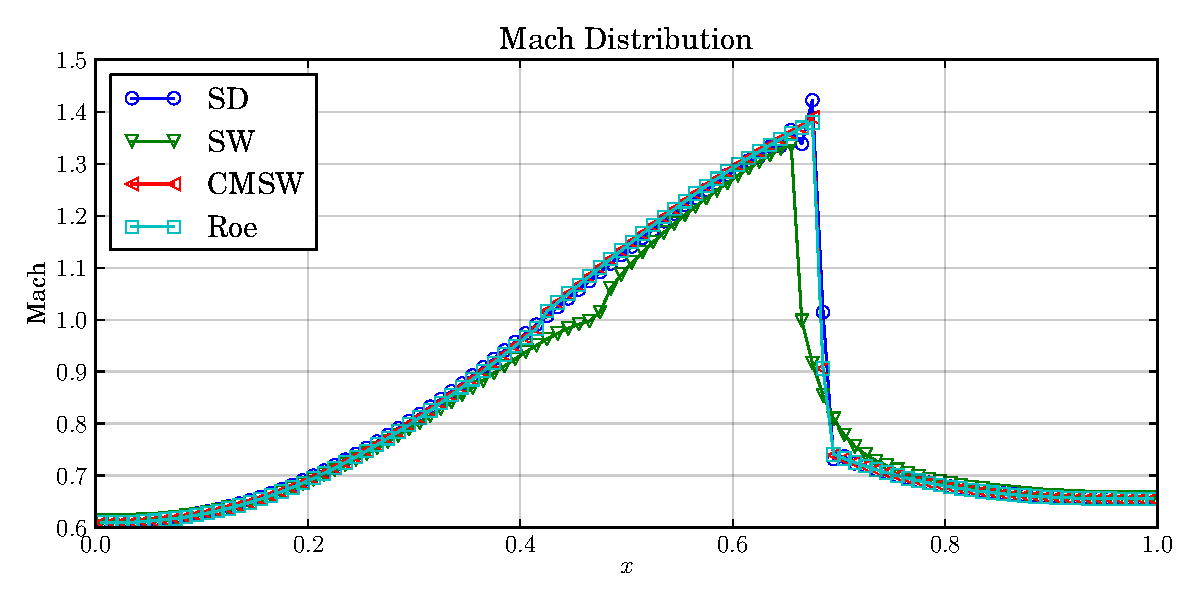
\includegraphics[width = 0.9\textwidth]{./figures/q4m.pdf}
    \caption {Mach Distribution for Various Flux Schemes}
    \label{fig:q4m}
\end{figure}

\begin{figure}[!ht]
    \centering
    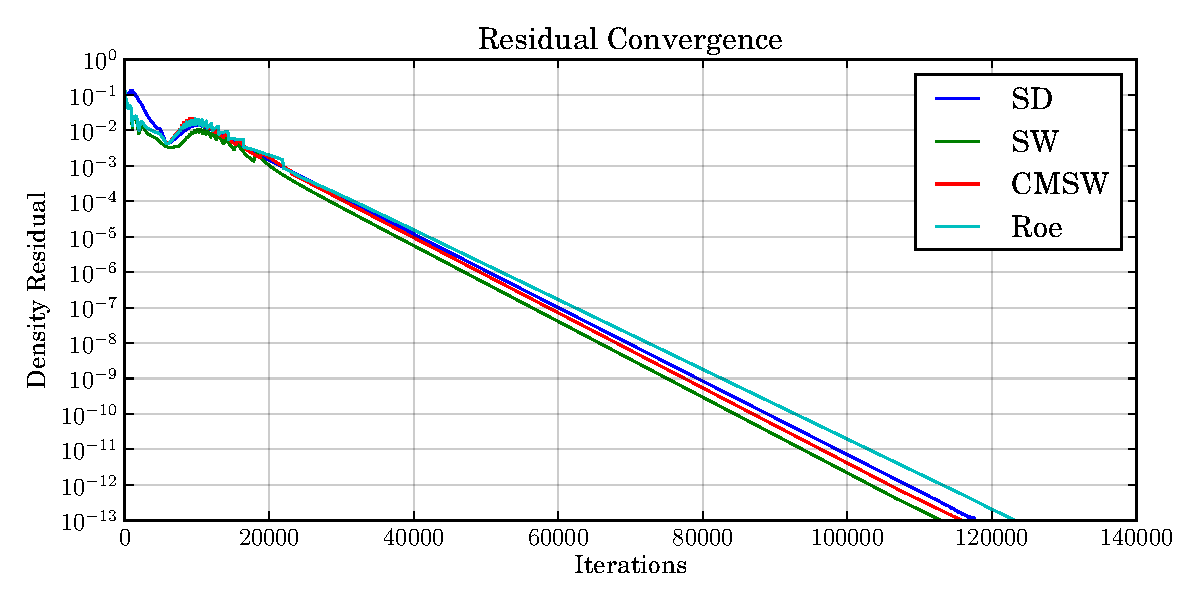
\includegraphics[width = 0.9\textwidth]{./figures/q4c.pdf}
    \caption {Density Residual Convergence for Various Flux Schemes}
    \label{fig:q4p}
\end{figure}

\begin{table}[!h]
\centering
\begin{tabular}{cc} \toprule
    {Flux Scheme} & {Total Pressure Loss} \\
    \midrule
    {SD}   & 0.0385511\\
    {SW}   & 0.0375228\\
    {MCSW} & 0.0395640\\
    {Roe}  & 0.0395788\\
\bottomrule
\end{tabular}
\caption{Total Pressure Loss for Various Flux Schemes}
\label{tab1}
\end{table}

\section{Time Discretization Study}

Roe flux scheme is used for spatial discretization.
Euler explicit uses a CFL of 0.95.
Runge-Kutta 4th order uses a CFL of 1.95.
Jameson's RK4 uses a CFL of 1.50.

\end{document}
